\documentclass[10pt,a4paper]{article}
\usepackage[utf8]{inputenc} % para poder usar tildes en archivos UTF-8
\usepackage[spanish]{babel} % para que comandos como \today den el resultado en castellano
\usepackage{a4wide} % márgenes un poco más anchos que lo usual
\usepackage{caratula}
% \usepackage[left=3cm,right=3cm,bottom=3cm,top=3cm]{geometry}

% Comandos para símbolos matemáticos.
\usepackage{amsmath, amssymb, tabularx}

% Comandos para referencias
\usepackage{natbib}
%listing /code
\usepackage{listings}

% Comandos para Figuras, Gráficos, Tikz etc.
\usepackage{tikz}
\usepackage{epsfig}
\usepackage{pgfplots}
\usepackage{graphicx}
\usepackage{epsfig}
\usepackage{caption}
\usepackage{subcaption}
\usepackage{svg}

% Comandos para teoremas etc.
\usepackage{amsthm}
\newtheorem{theorem}{Teorema}
\newtheorem{lemma}[theorem]{Lema}
\newtheorem{proposition}[theorem]{Proposición}
\newtheorem{remark}{Observación}
\newtheorem{corollary}{Corolario}
% \newproof{proof}{Demostración}

% Comandos para algoritmos.
\usepackage[noend]{algpseudocode}
\usepackage{algorithm}
\algnewcommand{\IfThenElse}[3]{% \IfThenElse{<if>}{<then>}{<else>}
\State \algorithmicif\ #1\ \algorithmicthen\ #2\ \algorithmicelse\ #3}
\algnewcommand{\IfThen}[2]{% \IfThenElse{<if>}{<then>}
  \State \algorithmicif\ #1\ \algorithmicthen\ #2}
  
\lstset{numberstyle=\tiny, stepnumber=1, numbersep=5pt, numbers=left,
    xleftmargin=.04\textwidth,
    breaklines=true,
    columns=fullflexible,
    flexiblecolumns=true,}
%\algrenewcommand{\algorithmiccomment}[1]{\hskip5em $\rightarrow$ #1}

\begin{document}

\titulo{TP2 - Problema de TSP}

\fecha{12 de julio de 2020}

\materia{Algoritmos y Estructuras de Datos III}

\integrante{Venegas, David Alejandro}{783/18}{davidalevng@gmail.com}
\integrante{Bustamante, Luis Ricardo}{43/18}{luisbustamante097@gmail.com}
\integrante{Castro, Jonatán Daniel}{63/18}{jonatan.dan@hotmail.com}
\integrante{Oshiro, Javier Esteban}{715/09}{javieroshiro@hotmail.com}

\maketitle

\newpage

\tableofcontents
\newpage
\setcounter{page}{1}

\section{Introducción} 

Los problemas de optimización combinatoria permiten modelar situaciones de la vida real, donde se debe tomar una decisión sobre un evento que repercute en una ganancia o un costo a pagar. En particular, los grafos permiten representar gran variedad de situaciones de amplio interés, como por ejemplo calcular horarios para hacer mantenimientos a servidores o la distribución de la mercancía en un \emph{warehouse} o depósito, así como el envió de productos y su respectivo ruteo. 

Actualmente, en un mundo cada vez más interconectado resulta de gran importancia resolver problemas de planificación y logística de forma eficiente, sin embargo, aun existe una limitante computacional para calcular la solución exacta (y probablemente siempre lo haga). Esto ocurre cuando se busca resolver un problema asociando una función objetivo al conjunto de posibles soluciones, debido a la gran la cantidad de comparaciones que se deben realizar para el conjunto de posibles instancias. Estos cálculos crecen de forma no polinomial para muchos de estos problemas, y por ello es necesario implementar heurísticas que permitan encontrar soluciones de forma eficiente (aunque no sean óptimas).

El problema del viajante de comercio (TSP por sus siglas en inglés) plantea el problema de un comerciante que debe recorrer un conjunto de ciudades, pasando por cada una exactamente una sola vez para luego regresar al origen realizando el mejor recorrido posible (que minimice la distancia recorrida, en este caso). Este problema es de los mas conocidos y estudiados en el mundo de la ciencias de la computación, por sus múltiples aplicaciones en la vida real, así como dificultad para alcanzar una solución exacta y su impacto económico, social y ambiental. 

En el presente trabajo práctico resolvemos este problema trasladándolo a grafos pesados de forma que la solución se obtiene al encontrar un circuito hamiltoniano de longitud mínima. En particular para este estudio por motivos prácticos se considera solo el caso de grafos completos, es decir cuando todas las ciudades están conectadas entre si. Para encontrar la  solución más eficiente (cercana al óptimo) en tiempo polinomial se emplearán heurísticas y meta-heurísticas para luego ser estudiadas y comparadas frente a diversos tipos de instancias.
%En especial se busca observar su comportamiento para instancias relacionadas con ciudades que tratan de modelar el mundo real y en particular permiten con una cantidad de paradas adecuadas para tratar de calcular el mejor recorrido para un repartidor de envíos en un día normal. 
Por último, para las meta-heurísticas se busca la mejor combinación posible de parámetros y heurísticas bases a fin de obtener como aplicación práctica de la presente investigación un algoritmo capaz de conseguir una solución eficiente, aunque no exacta, al problema del TSP. Esta selección sera una consecuencia de la experimentación empírica con las instancias mencionadas comparando el gap entre la solución obtenida y el óptimo en cuestión.  

\subsection{Travelling Salesman Problem (TSP)}

Es difícil marcar el origen del TSP, pero se estima que el problema fue tratado por primera vez en 1800 por el matemático irlandés W. R. Hamilton y el británico Thomas Kirkman. De acuerdo a Hoffman y Wolfe (1985, p. 5), su primera mención bibliográfica fue en un libro para viajantes de comercio de 1832 que incluía ejemplos de rutas entre Alemania y Suiza pero no incluía aproximaciones formales. Este problema no fue definido matemáticamente sino hasta 1930s donde Karl Menger describe el problema y considera por primera vez la solución por fuerza bruta y la heurística del vecino más cercano. Desde entonces, con el paso de los años el TSP despertó el interés de la comunidad científica y se convirtió en uno de los problemas mas estudiados de la computación, con constantes avances en especial en las ultimas 5 décadas, y cuyo impacto fue el ahorro de billones de dolares al optimizar diversas ramas de la industria, desde envíos, y protocolos de comunicación, entre muchas otras. 

Formalmente, se plantea que dado un grafo \boldmath$G=(V,X)$ con longitudes asociadas a sus aristas $l: X \rightarrow R \geq 0$, queremos determinar un circuito hamiltoniano $C^0$ tal que $l(C^0)=min\{l(C)|C\ es\ circuito\ hamiltoniano\ de\ G\}$. \cite{teo:Hamiltoniano}

Actualmente no se conocen algoritmos polinomiales para resolver este problema y tampoco $e$-aproximados polinomiales para el caso general (sin distancias euclidianas) ya que este es un problema NP-difícil (y quizás nunca se conozcan). La complejidad del algoritmo \emph{naive} para resolver el TSP es de $O(n!)$, por lo que con un número de vértices mayor a 10 la cantidad de posibles permutaciones asciende a más de 300mil, y para un n grande puede tardar siglos en encontrar la solución exacta, otras soluciones utilizando programación dinámica pueden conseguir una solución óptima en $O(n^2*2^n)$, lo cual es una mejora considerable pero aun no es una solución computacionalmente eficiente o bien resuelta (sigue siendo exponencial). Sin embargo, hoy en día en la práctica se ha logrado desarrollar programas capaces de resolver este problema para instancias de hasta 85900 vértices. Esto se produjo en abril de 2006 mediante el programa TSP Concorde\cite{teo:concorde} usando 136 años de CPU en una computadora con 2.4GHz AMP Opterons distribuida en 250 nodos. Actualmente para instancias con millones de ciudades se puede encontrar soluciones con un 1\% de diferencia con la solución óptima.  

\subsection{Aplicaciones en la industria}

Dado que existen tantos problemas de optimización que se modelan de forma similar al TSP, encontrar una forma mas eficiente de resolverlo es de suma importancia. Algunos ejemplos son: \unboldmath

Proyecto ORION (por sus siglas en ingles para \emph{Onroad Integrated Optimization and Navigation}) en un software desarrollado por la compañía de envíos norteamericana UPS (United Parcel Service), el cual tras décadas de desarrollo permite calcular las rutas para la flota de más de 58000 camiones que por día que emplea UPS en sus entregas, los cuales hacen cerca de 130 paradas o entregas cada uno. Se estima que por cada milla que ORION esta más cerca de la solución óptima, es decir por cada milla que cada camión ahorra por día,  UPS ahorra 50 millones de dolares \cite{teo:ups}. 

Otra aplicación a la solución del problema TSP es en la optimización de la producción de tableros para circuitos integrados (PCB por sus siglas en inglés).
Hoy en día se fabrican cientos de millones de electrónicos todos los años, los cuales en su mayoría requieren de al menos un PCB para su fabricación. Siendo esta industria tan masiva cualquier aumento en la productividad tiene una repercusión económica significativa, por lo cual se suelen aplicar algoritmos con heurísticas especializadas para optimizar este proceso, no solo en el tiempo y recorrido de la maquina para perforar los circuitos sino tomando otras restricciones \emph{novel-friendly} que tienen en cuenta tanto el margen de error del taladro como la durabilidad de sus componentes al tratar de calcular rutas casi óptimas\cite{teo:PCB}. Este problema también se puede trasladar a la planificación del proceso de integración y soldado de los componentes en el tablero. 
\begin{figure}[h!]
    \centering
    \centering
    \begin{tabular}{c c}
        \textbf{\underline{Solución en la Industria}} & \textbf{\underline{Solución Óptima}} \\
        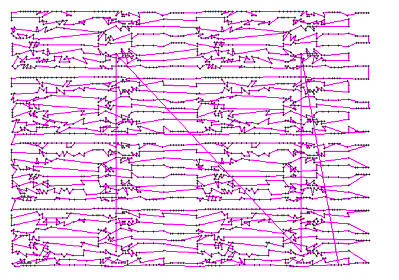
\includegraphics[scale=0.5]{img/tsp1.png} & 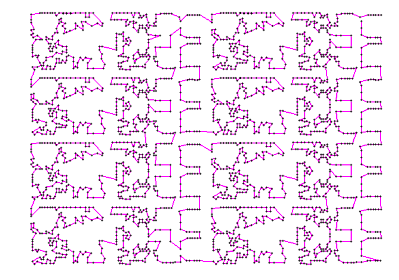
\includegraphics[scale=0.5]{img/tsp2.png}
    \end{tabular}
    \captionsetup{justification=centering}
    \caption{Aplicación del TSP en el perforado de PCBs}%
    \label{fig:sol_ind}%
\end{figure}

Ahora, enfocando el TSP desde el marco de estudio del proyecto es necesario empezar por resolverlo mediante el uso de heurísticas \cite{teo:Heuristicas} para obtener una solución satisfactoria y eficiente en el tiempo, pero no necesariamente óptima. A partir de esta solución inicial se pueden aplicar técnicas de meta-heurísticas para tratar de mejorar el resultado encontrado. A continuación se exploran estas técnicas.

%-------------------SECTION DESARROLLO ------------------------------------------------
\newpage
\section{Heurísticas}

Las heurı́sticas constructivas son métodos que permiten construir una solución posible solución para una instancia de un problema. No garantiza encontrar la mejor solución e incluso podría generar una solución válida aleatoria. Por su facilidad de diseño e implementación son utilizados frecuentemente.

%--------------------- START HEURISTICA VECINO MAS CERCANO--------------------
\subsection{Heurística de vecino más cercano}
Es un algoritmo goloso que toma un grafo representado como una lista de adyacencias y partiendo del primer vértice de la entrada calcula un circuito hamiltoniano agregando en cada iteración el vértice vecino más cercano aún no recorrido, hasta completar el ciclo hamiltoniano.

\begin{algorithm}
	\begin{algorithmic}[1]
		\Function{$heuristica\_vmc$}{$grafo\ G$}
		\State $vActual \leftarrow G[0]$ \Comment $O(1)$
		\State $camino \leftarrow crearListaVacia()$  \Comment $O(1)$
		\State  $agregar(camino, vActual)$  \Comment $O(1)$
		\While{$camino.size() < G.size()$}
		        \State $vActual \leftarrow vMasCercanoNoVisitado(vActual)$ \Comment $O(n)$
		        \State $agregar(camino, vActual)$ \Comment $O(1)$
		\EndWhile
		\State \textbf{return} $camino$.

		\EndFunction
	\end{algorithmic}
	\caption{Heurística de vecino más cercano.}
	\label{alg:hvmc}
\end{algorithm}

Vemos en el código \ref{alg:hvmc} que $vMasCercanoNoVisitado$ es una función que devuelve el vecino más cercano del vértice actual que no haya sido visitado en alguna de las iteraciones anteriores.

\subsubsection{Complejidad}
Las primeras lineas del algoritmo tienen complejidad $O(1)$, si es que la variable camino se inicializa como una lista y no como un vector de $n$ posiciones. Aún si camino fuese inicializada como vector, sería irrelevante para ver la complejidad, pues encontraremos que ella resulta ser $O(n^2)$.
Para recorrer todos los vértices, es necesario y suficiente que se ejecuten $n$ iteraciones del while, por lo cual su complejidad teniendo en cuenta lo que está adentro de él será $O(n)$ multiplicado por $O(interior\ del\ while)$. 

Evaluemos lo que hay dentro del while: $agregar$ es una función que coloca en la última posición de camino el vértice actual, y por ser la implementación una lista, se ejecuta en $O(1)$. La función $vMasCercanoNoVisitado$ recorre todos los vértices adyacentes al actual. La peor situación en órdenes de complejidad para la función en el caso general es cuando el vértice actual es adyacente a todos los del grafo, y en particular para el presente TP esto siempre ocurre ya que se utilizan grafos completos, resultando así en $O(n-1)$ al chequearlos todos.
Por esto, la complejidad del $while$ es $O(n) . O(n)$, que es igual a $O(n^2)$, siendo esta última la complejidad de la heurística.

\subsubsection{Casos patológicos}

Para la heurística de vecino más cercano podemos considerar una instancia patológica donde en principio se tiene un grafo euclideano, donde las artistas y vértices respetan la desigualdad triangular, a excepción de una arista, que tiene el peso mayor a la suma del peso de todas las demás. El caso patológico, entonces, está dado cuando el algoritmo hace un camino hamiltoniano y en el último vértice a la hora de conectarlo con el primero, se utiliza la arista de peso anormal para cerrar el circuito. Claramente si hubiésemos colocado al vértice en otra posición del camino armado, usaríamos otras aristas que nos proporcionarían un peso del circuito mucho menor.

\begin{figure}[!h]
    \centering
    \captionsetup{justification=centering}
    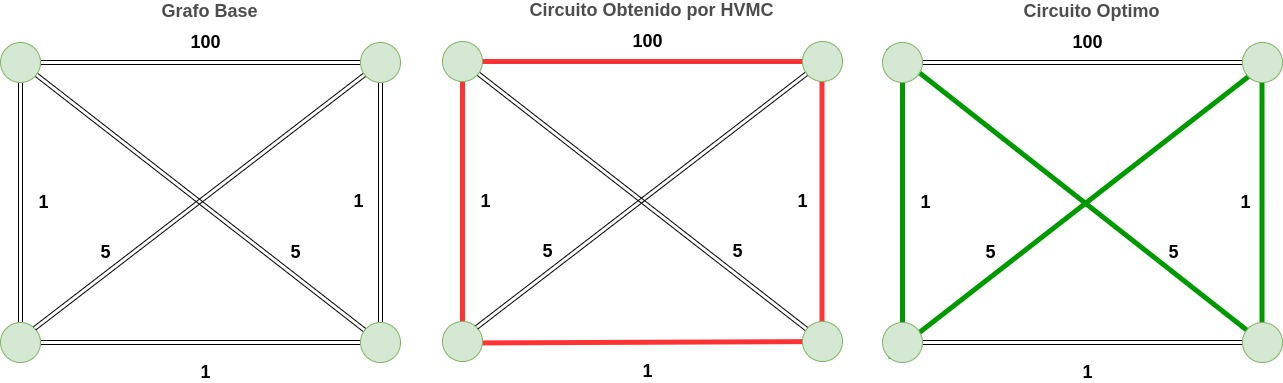
\includegraphics[scale=0.3]{Graphs/mal caso HVMC.jpg}
    \caption{Comparación Circuito Óptimo VS Circuito encontrado en HVMC}
    \label{fig:hvma_patologico}
\end{figure}
%--------------------- END HEURISTICA VECINO MAS CERCANO--------------------
\subsection{Heurística de la arista más chica} \label{sec:hamc}

Esta técnica se basa en hacer uso del concepto detrás del algoritmo de Kruskal al revisar si se forma o no un ciclo  antes agregar vértices, pero trasladado al problema de encontrar un circuito hamiltoniano. Esta heurística se basa en seleccionar en cada iteración la arista de menor peso tal que ningún vértice tenga grado mayor a 2 y no se formen ciclos antes de recorrer todos los vértices, por lo cual su comportamiento también es goloso al igual que la anterior. Para su implementación se utiliza una lista de incidencia para representar el grafo y una estructura \emph{Union-Find} para representar las partes conexas del mismo, en particular esta última permite disminuir las operaciones necesarias para revisar si al agregar un arista se forma un ciclo, y dado que este ocurre en cada iteración esta optimización es significativa para la complejidad final del algoritmo. Específicamente se utiliza una unión por rangos, además de la compresión de caminos según lo visto en el laboratorio de la materia, esto último es particularmente útil en la función \emph{esCiclo}. A continuación se expresa el pseudocódigo de la heurística:

\begin{algorithm}
	\begin{algorithmic}[1]
		\Function{$heuristica\_aristaMasCorta$}{$grafo\_list\_Inc\ G$, $int\ n$ , $lista\ H$}
		\State $G \leftarrow ordenar(G)$ \Comment $O(n^2log(n^2)$
		\State $grados \leftarrow crear\_lista(0,n)$  \Comment $O(n)$
		\State $i \leftarrow 0$  \Comment $O(1)$
		%\State $hay\_ciclo \leftarrow False $, $hay\_nodo\_grado3 \leftarrow False$
		\While{$aristas.size() < n$}
            \If{$\neg hay\_nodo\_grado3()$} \Comment $O(1)$     
                %\State$ vertices\_temp \leftarrow vertices + cant\_nodos\_nuevos()$ \Comment $O(1)$ 
                \State $aristas \leftarrow agregar(G[i])$ \Comment $O(n)$ 
		        \State $hay\_ciclo \leftarrow esCiclo(aristas, n)$ \Comment $O(n* \alpha(n))$
		    \If{$hay\_ciclo$}
		        \State $aristas \leftarrow quitar(G[i])$ \Comment $O(n)$
		    \Else
		        %\State $vertices \leftarrow vertices\_temp$ \Comment $O(1)$
		        \State $incrementar(grado[G[i].src])$ \Comment $O(1)$
                \State $incrementar(grado[G[i].dest])$ \Comment $O(1)$
            \EndIf
            \EndIf
		\State $incrementar(i)$ \Comment $O(1)$
		\EndWhile
		\State $construir\_circuito(aristas)$ \Comment $O(n^2)$
		\State \textbf{return} $suma(aristas)$.
		\EndFunction
	\end{algorithmic}
	\caption{Heurística de la arista más chica.}
	\label{alg:hamc}
\end{algorithm}

El algoritmo inicialmente ordena la lista de incidencia según el peso de cada arista y luego busca generar una lista de aristas que conformará el circuito hamiltoniano. Inicialmente esta lista se encuentra vacía y se itera hasta llenarla con $n$ aristas (las necesarias para armar un circuito hamiltoniano). Antes de agregar cada arista se utiliza la función \texttt{hay\_nodo\_grado3()} para revisar que el grado de ambos vértices de la arista no sea mayor o igual a $2$. Si el grado de los vértices es valido, agrega el vértice a la lista \emph{aristas}. Luego ejecuta la función \texttt{esCiclo(aristas,n)} para determinar si se forma un ciclo al agregar la arista, de hacerlo se elimina la arista agregada, sino se mantiene esta y se incrementa el grado de ambos vértices de la arista en cuestión. Se incrementa $i$ para seguir iterando hasta terminar el ciclo, y finalmente se construye el circuito de vértices a partir de la lista de aristas no ordenadas. Por último se suman los pesos de la aristas para obtener el costo final del circuito. 

\subsubsection{Complejidad}

El primer ordenamiento tiene un costo de $O(n^2log(n^2))$ ya que sabemos que es un grafo completo y tiene $m$ aristas tal que $m=n(n-1)$. En el ciclo \emph{while} se iteran $n$ veces a lo sumo, y la operación mas costosa es decidir si hay un ciclo la cual toma $O(n.\alpha(n))$ donde $\alpha$ es la inversa de la función de Ackerman, esto corresponde a las operaciones de \emph{Union} y \emph{Find} usadas en la función. Luego agregar o quitar aristas es $O(1)$ amortizado, pero en el pseudocódigo se señala el peor caso en $0(n)$, por lo cual el costo del ciclo sería $O(n^2*\alpha(n))$. Finalmente, construir el circuito se hace en $O(n^2)$ y la suma del peso de las aristas en $O(n)$. Por todo lo mencionado anteriormente la complejidad final de la heurística es  $O(n^2log(n^2) + n^2\alpha(n))$ que es equivalente a $O(n^2log(n^2))$.

\subsubsection{Casos patológicos}

Para este algoritmo al igual que con el HVMC existe un mal caso siempre que la última arista con el que se cierra el ciclo tenga un valor superior al peso total del circuito óptimo. De esta forma se obtiene una solución casi 100\% mayor a la ideal, y como siempre se parte del primer vértice se pueden construir circuitos tan lejos del óptimo como uno quiera. Sumado a esto, existen familias de grafos que se pueden construir para que el circuito resultante se acerque al peor caso posible, esto se hace explotando la vulnerabilidad de que el algoritmo goloso no revisa soluciones previas, por lo cual a partir de un cierto vértice $k$ la arista óptima apunta a un vértice ya recorrido, por lo cual se descarta y se selecciona una de las disponibles. En particular las aristas restantes deben ser de costo elevado para alejarse los máximo posible del óptimo. Construir estas instancias para mapas grandes no es trivial y es poco frecuente en el mundo real por lo cual no se experimentará directamente sobre ellas por razones prácticas. Por ultimo, es interesante destacar que esta heurística se puede combinar con técnicas de programación lineal para tratar de acotar a priori si un tour o recorrido va a dar un buen resultado.\cite{teo:pe}

\subsection{Heurística del árbol generador} \label{sec:hagm}
En este método primero se busca generar un AGM (árbol generador mínimo) mediante un algoritmo conocido (en nuestro caso usamos el método de Prim \cite{teo:Arboles}), luego obtenemos el orden de recorrido de los vértices al aplicar DFS \cite{teo:Arboles} sobre el árbol, y finalmente siguiendo este orden generamos el circuito hamiltoniano.
Este método tiene la característica de que es $1$-aproximado en el caso de grafos euclideanos (todas sus aristas cumplen desigualdad triangular).

\begin{algorithm}
	\begin{algorithmic}[1]
		\Function{$heuristica\_agm$}{$grafo\ G, lista\ H$}
		
		\State $T \leftarrow agm\_prim(G)$ \Comment{$O(n^2)$}
		\State $H \leftarrow orden\_dfs(T)$ \Comment{$O(n^2)$}
		\State $P \leftarrow calcular\_peso(H)$ \Comment{$O(n^2)$}
		\State \textbf{return} $P$.

		\EndFunction
	\end{algorithmic}
	\caption{Heurística de árbol generador.}
	\label{alg:hagm}
\end{algorithm} 	

En el pseudocódigo \ref{alg:hagm} la función recibe como entrada el grafo $G$, y por referencia una lista $H$ donde se devuelve el circuito hamiltoniano. La función $agm\_prim$ genera el AGM utilizando el método de Prim, $orden\_dfs$ genera una secuencia de vértices que se condicen con el órden recorrido por el método DFS sobre el AGM obtenido, este es nuestro circuito hamiltoniano. Y finalmente $calcular\_peso$ calcula el peso del circuito hamiltoniano.

\subsubsection{Complejidad}
En $agm\_prim$ usamos la implementación con listas pues es eficiente cuando el grafo es completo (denso). Esta tiene complejidad $O(n^2)$ según lo visto en la clase de laboratorio de AGM \cite{lab:AGM}.

En $orden\_dfs$ debemos recorrer el árbol completo en $O(n)$, pero por cada vértice debemos elegir un hijo para continuar el recorrido. Como utilizamos una estructura $padre[i]$ que tiene en cada posición quién es el padre del vértice $i$, elegir un hijo que todavía no fue tenido en cuenta lo hacemos en $O(n)$. Finalmente tenemos complejidad $O(n^2)$.

En $calcular\_peso$ debemos recorrer los $n$ vectores del circuito y por cada uno obtener el peso de la arista lo une con el siguiente. Como tenemos una estructura de lista de adyacencia, encontrar el peso de la arista es $O(n)$ pues el grafo es completo. Finalmente lo hacemos con complejidad $O(n^2)$.

La complejidad total de la heurística es $O(n^2 + n^2 + n^2) \in O(n^2)$.

\subsubsection{Casos patológicos}
Sabemos que existen instancias donde la garantía del algoritmo de ser 1-aproximado no se cumple. Esto pasa cuando las aristas no representan distancias euclideanas (no se respeta la desigualdad triangular), luego existen vértices para los cuales ir directo cuesta más que hacer un salto por un vértice intermedio. En estos casos podemos generar instancias donde el peso de las aristas que unen los vértices del DFS sea mucho mayor que algún otro circuito hamiltoniano existente que no siga ese orden.

\section{Metaheurística Tabú Search}
Está basada en la idea de encaminar la búsqueda de soluciones evitando quedar atrapado en un óptimo local. Es un algoritmo iterativo similar a la búsqueda local en el que a partir de una solución inicial se evalúa un subconjunto de soluciones factibles llamado Vecindad, obtenido a partir de realizar movimientos (variaciones entre vértices) sobre el circuito generado en cada paso.
Para obtener la solución inicial vamos a utilizar la heurística de árbol generador mínimo pues como vimos en la sección \ref{alg:hagm} es 1-aproximada para grafos con distancias euclideanas lo que nos da una garantía de calidad.
Utiliza una estructura de memoria de tamaño fijo (configurada como parámetro) que permite detectar si una solución ya fue considerada en una iteración anterior del algoritmo, evitando caer en loops de soluciones factibles.
Al ser un algoritmo que puede demorar mucho tiempo de ejecución si revisamos todas las soluciones, utilizamos criterios de parada del ciclo principal devolviendo como solución la mejor encontrada hasta el momento. 
Los criterios de parada utilizados son: cantidad de iteraciones totales, cantidad de iteraciones sin mejora de solución, y tiempo de ejecución.
Además, se tienen dos tipos de memoria seleccionables para este algoritmo, una basada en memorizar ciclos para no tenerlos en cuenta mientras busco futuras vecindades, y otra basada en memorizar intercambios de aristas, es decir no volver a analizar aristas que ya fueron descartadas durante el armado de la vecindad. 

\begin{algorithm}
	\begin{algorithmic}[1]
		\Function{$tabuSearch$}{$grafo\ G, lista\ H$}
		
		\State $c \leftarrow heuristica\_agm(G)$ \Comment{$O(n^2)$}
		\State $c^* \leftarrow c$
		\State $m \leftarrow inicializar\ memoria$
		
		\While{$!criterioParada()$}
            \State $V \leftarrow obtenerVecindad(c^*)$ \Comment{$O(n^3)$}
            \State $c' \leftarrow min\{c' \in V : pesoCircuito(c') < pesoCircuito(cv) \forall cv \in V$\} \Comment{$O(n^3)$}
            \State $actualizarMemoria(m, c)$
            
            \If{$pesoCircuito(c') < pesoCircuito(c^*)$} \Comment{$O(n)$}
                \State $c^* \leftarrow c'$
            \EndIf
		\EndWhile
		\State $H \leftarrow c^*$
		\State \textbf{return} $pesoCircuito(c^*)$.

		\EndFunction
	\end{algorithmic}
	\caption{Metaheurística Tabu Search.}
	\label{alg:mheur}
\end{algorithm} 	

\subsection{Complejidad}
Ya vimos anteriormente en la sección \ref{sec:hagm} que la heurística de AGM tenía complejidad $O(n^2)$.

La función $obtenerVecindad()$ se encarga de generar el subconjunto de ciclos vecinos realizando movimientos 2-opt y guardando solo los que mejoran el ciclo actual. De estos sólo consideramos un porcentaje parametrizado. Como se analiza realizar el movimiento 2-opt de todos los vértices contra todo el resto, se puede recorrer todas las posibilidades en $O(n^2)$. Cada swap 2-opt implica rearmar el ciclo, luego tiene complejidad $O(n)$. Finalmente tenemos complejidad $O(n^3)$ para esta función. 

La función $pesoCircuito()$ calcula la sumatoria de los pesos de todas las aristas del circuito en $O(n)$. Luego obtener el mínimo ciclo pesado en la vecindad $V$ es $O(|V| * n)$. Como la vecindad tiene como mucho $n^2$ ciclos a los que se les aplicó movimiento 2-opt, entonces la complejidad es $O(n^3)$.

La función $actualizarMemoria()$ simplemente agrega un nuevo elemento a la lista memoria en $O(1)$.

La comparación de pesos de ciclos en la linea $9$ del pseudocódigo \ref{alg:mheur} podemos hacerla en $O(1)$ recibiendo el peso de cada ciclo de sus respectivas funciones que lo generan, sin necesidad de volver a calcularlo. En todo caso volver a calcularlo podemos hacerlo en $O(n)$ cada ciclo, lo que no agrega complejidad adicional en el algoritmo general.

Dado que revisar todas las posibilidades hace que sea impracticable correr el algoritmo por cuestiones de tiempo de ejecución, el ciclo principal se ejecuta una cantidad de veces acotada por parámetros fijos independientes del tamaño del grafo de entrada obteniendo complejidad teórica constante. Sin embargo podemos analizar el costo computacional por cada iteración del ciclo principal del algoritmo y podemos ver que la complejidad teórica por ciclo es $O(n^2 + n^3 + n^3 + n) \in O(n^3)$.

\newpage    
\section{Experimentación}
Los siguientes experimentos fueron corridos todos en una única máquina de características: procesador Intel i3-6100u 2.3 Ghz 3 Mb Cache L3, y memoria RAM de 6 GB DDR4. En los experimentos de complejidad consideramos la media de 5 ejecuciones para mayor fidelidad de tiempo, en el resto de los experimentos se realizó una única ejecución por motivos prácticos a razón de las múltiples horas de cómputo que requirieron los experimentos. 

\subsection{Instancias}\label{sec:exp-instancias}
Para las siguientes experimentaciones utilizamos distintos conjuntos de instancias específicos para los objetivos de cada experimento.

Durante el análisis de complejidad de los algoritmos utilizamos grafos completos pesados de tamaño variable hasta 50 vértices. Dado que solo nos interesa el tiempo de cómputo y no el resultado, podemos usar aristas de pesos semi-aleatorios sin ninguna consecuencia sobre el rendimiento. El peso de cada arista $(i, j)$ de este conjunto esta dado por la fórmula $((i+1)*(j+1))\ mod\ 100)$.

Para evaluar la calidad de las heurísticas, a fines prácticos seleccionamos el conjunto de instancias conformado por mapas de ciudades reales, donde cada vértice representa una parada o ubicación. Para ello seleccionamos un subconjunto de las disponibles en TSPLIB \cite{web:tsplib} que sean euclidianas, fáciles de parsear e incluyen su solución óptima al problema de TSP expresada en el peso total de los vértices del circuito hamiltoniano mínimo. Estas mismas se utilizaron a su vez para evaluar las meta-heurísticas y sus mejores parámetros para este caso de estudio. A continuación las instancias que empleamos son:
\begin{itemize}
    \item 'berlin52': problema de 52 ubicaciones en Berlín. Solución óptima: $7542$.
    \item 'eil51': problema de Christofides/Eilon de 51 ubicaciones en una ciudad. Solución óptima: $426$.
    \item 'eil76': problema de Christofides/Eilon de 76 ubicaciones un una ciudad. Solución óptima: $538$.
    \item 'kroA100': problema de Krolak/Felts/Nelson de 100 ubicaciones en una ciudad. Solución óptima: $21282$.
    \item 'st70': problema de Smith/Thompson de 70 ubicaciones un una ciudad. Solución óptima: $675$.
\end{itemize}

Las siguientes instancias serán usadas para poner a prueba el rendimiento de los valores óptimos (empíricos) que obtendremos durante la etapa de experimentación con parámetros, como se pide en el punto 5 del enunciado.
Esta ultima se diferencia del resto solo en lo que representa ya que se trata de grafos en forma de grilla.
\begin{itemize}
    \item 'rat195': problema de Pulleyblank. Solución óptima: $2323$.
    \item 'rat575': problema de Pulleyblank. Solución óptima: $6773$.
    \item 'rat783': problema de Pulleyblank. Solución óptima: $8806$.
\end{itemize}

%\newpage %newpage porque sino los graficos quedan colocados en mal lugar
\subsection{Complejidad de heurística vecinos más cercanos}
Para poner a prueba nuestra hipótesis de que la complejidad insumida por la heurística del vecino más cercano es efectivamente $O(n^2)$, tomamos un dataset de grafos con aristas definidas según lo mencionado en la sección \ref{sec:exp-instancias}. No hicimos uso de los casos patológicos del punto 4.c del enunciado, pues están relacionados a la calidad de la solución, no a la complejidad, sin embargo es interesante destacar que para el caso de grafos completos como cada vértice tiene $n-1$ aristas y estas siempre se deben recorrer para asegurarnos de encontrar el mínimo, se puede establece una cota inferior $\Omega(n^2)$. 

Corrimos instancias del dataset con tamaños del 5 al 50, un total de 5 veces cada instancia y tomamos la media, de forma que tengan mejor precisión las mediciones.

\begin{figure}[h!]
    \centering
    \captionsetup{justification=centering}
    \begin{subfigure}{0.45\linewidth}
        \includesvg[scale=0.45]{Graphs/H1-complejidad-2}
        \centering
        \caption{Tiempo de ejecución de HVMC frente a $O(n^2)$.}
        \label{fig:exp_hvmc_1}
    \end{subfigure}
    \begin{subfigure}{0.45\linewidth}
        \centering
        \includesvg[scale=0.45]{Graphs/H1-correlacion}
        \caption{Correlación de Pearson de la ejecución con HVMC.}
        \label{fig:exp_hvmc_2}
    \end{subfigure}
    \caption{Comparaciones con la complejidad esperada con HVMC.}
\end{figure}

En la Figura \ref{fig:exp_hvmc_1} contrastamos el tiempo transcurrido de correr las instancias contra una parábola de la forma $O(n^2)$, y se presentaron unos pocos outliers mayores a lo que esperábamos, una hipótesis sobre estos es que se deban a interrupciones del sistema operativo u otros procesas en la maquina donde se realizaron los experimentos, sin embargo corroboramos que la complejidad es la correcta en la segunda gráfica, donde se visualiza la correlación de Pearson entre lo esperado y lo obtenido con un valor de aproximadamente $0.962$.

En efecto, podemos ver que que se confirma la hipótesis sobre la complejidad, es decir que los resultados se asemejan a la curva esperada y en la Figura \ref{fig:exp_hvmc_2} se aprecia una correlación directa entre las variables mencionadas. 
\newline

\subsection{Complejidad de heurística de la arista mas corta} \label{sec:exp-hamc-complejidad}

En la Sección \ref{sec:hamc} explicamos el uso de la heurística de la arista mas corta (HAMC) en la cual concluimos que su complejidad era de $O(n^2*log(n^2))$, mediante el mismo conjunto de instancias que usamos en la sección anterior llamado \emph{completos-random}, también procedimos a correr las instancias de la misma forma, es decir 5 veces por instancia con grafos completos de tamaño 5 a 50.
\begin{figure}[h!]
    \centering
    \captionsetup{justification=centering}
    \begin{subfigure}{0.45\linewidth}
        \centering
        \includesvg[scale=0.5]{Graphs/H2-complejidad-2}
        \caption{Tiempo de ejecución de HAMC frente a $O(n^2*log(n^2))$.}
        \label{fig:exp_hamc_1}
    \end{subfigure}
    \begin{subfigure}{0.45\linewidth}
        \centering
        \includesvg[scale=0.5]{Graphs/H2-correlacion}
        \caption{Correlación de Pearson de la ejecución con HAMC.}
        \label{fig:exp_hamc_2}
    \end{subfigure}
    \caption{Comparaciones con la complejidad esperada con HAMC.}
\end{figure}

En la Figura \ref{fig:exp_hamc_1} podemos ver como los tiempos de ejecución de la heurística se ajusta a medida que crece $n$ con la complejidad esperada. 
Igual que en el caso anterior, la cantidad de outliers no es significativa y la correlación de los datos esperados y obtenidos se puede terminar de verificar con la Figura \ref{fig:exp_hamc_2} donde se obtuvo un índice de Pearson de aproximadamente $0.992$.

Vale la pena destacar que a pesar de tener una complejidad mayor a las otras heurísticas, siendo que el $O(n^2log(n^2)$ de la complejidad viene del ordenamiento inicial, tenemos tiempos incrementalmente bajos con respecto a los de una implementación \emph{naive} del problema.
Aun así no es de las heurísticas mas eficientes en tiempo, como se muestra más adelante en otra experimentación.
%\newpage %newpage porque sino los graficos quedan colocados en mal lugar
\subsection{Complejidad de heurística del árbol generador mínimo}
Hasta ahora vimos los resultados de dos heurísticas basadas en conceptos mas sencillos de implementar, en este sección mostraremos los resultados de la heurística del árbol generador mínimo (o HAGM) la cual como fue detallado en la sección \ref{sec:hagm} esta basada en el algoritmo de Prim, y además se mostró que la complejidad del algoritmo es $O(n^2)$. Se utiliza el mismo conjunto de instancias que en los experimentos anteriores, con la misma cantidad de ejecuciones por instancia e igual $n$ mínimo y máximo.

\begin{figure}[h!]
    \centering
    \captionsetup{justification=centering}
    \begin{subfigure}{0.45\linewidth}
        \centering
        \includesvg[scale=0.5]{Graphs/HAGM-complejidad-2}
        \caption{Tiempo de ejecución de HAGM frente a $O(n^2)$.}
        \label{fig:exp_hagm_1}
    \end{subfigure}
    \begin{subfigure}{0.45\linewidth}
        \centering
        \includesvg[scale=0.5]{Graphs/HAGM-correlacion}
        \caption{Correlación de Pearson de la ejecución con HAGM.}
        \label{fig:exp_hagm_2}
    \end{subfigure}
    \caption{Comparaciones con la complejidad esperada con HAGM.}
\end{figure}

Podemos ver que por la Figura \ref{fig:exp_hagm_1} que se respeto lo que esperábamos, a pesar de ver algunos puntos un poco fuera del rango esperado, esto puede ser debido al ruido del sistema al momento de ejecutarse las pruebas, aun así tenemos una complejidad que es respetada por los resultados del experimento, esto es acompañado de la Figura \ref{fig:exp_hagm_2} donde el índice de correlación de Pearson obtenido fue de aproximadamente $0.964$ corroborando la complejidad planteada.

%Es destacable que la heurística tiene valores de tiempo bastante bajos, y luego en próximos experimentos, veremos que además de tener un buen rendimiento tiene resultados cercanos al óptimo para conjuntos de instancias determinados, además de una cota con respecto al óptimo para grafos euclidianos.

\subsection{Comparaciones entre heurísticas}
Con el objetivo de comparar tiempos de ejecución y calidad del resultado (cercanía con el óptimo) vamos a evaluar un conjunto de 5 instancias para las cuales conocemos sus soluciones óptimas reales. Estas instancias son: 'berlin52', 'eil51', 'eil76', 'kroA100', y 'st70' ya mencionadas en la sección \ref{sec:exp-instancias}. La hipótesis es que la heurística de AGM debe dar mejor en general, pues garantiza una solución 1-aproximada para grafos euclidianos como vimos en la sección \ref{alg:hagm}.

\begin{figure}[h!]
    \centering
    \captionsetup{justification=centering}
    \begin{subfigure}{0.45\linewidth}
        \centering
        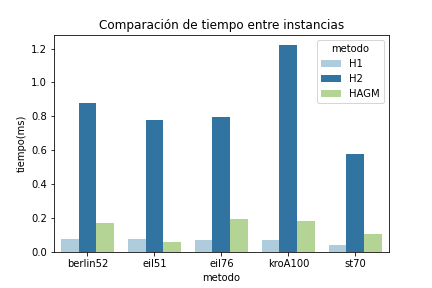
\includegraphics[scale=0.5]{Graphs/heur-tiempo.png}
        \caption{Tiempos de ejecución.}
        \label{fig:exp_heur_tiempo}
    \end{subfigure}
    \begin{subfigure}{0.45\linewidth}
        \centering
        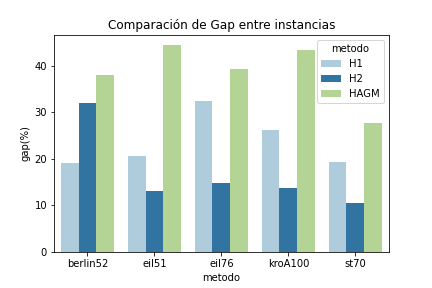
\includegraphics[scale=0.5]{Graphs/heur-gap.png}
        \caption{Calidad de las soluciones.}
        \label{fig:exp_heur_gap}
    \end{subfigure}
    \caption{Comparaciones entre heurísticas.}
\end{figure}

En la Figura \ref{fig:exp_heur_tiempo} se muestran los tiempos de ejecución en milisegundos, y a la derecha en la Figura \ref{fig:exp_heur_gap} se muestra el gap relativo entre la solución obtenida y la óptima. El método 'H1' se corresponde con la heurística de vecino más cercano, 'H2' con la heurística de arista más corta, y 'HAGM' con la heurística de árbol generador mínimo.

Podemos observar que la heurística de arista más corta demora mucho más tiempo que las otras dos. Esto refleja lo visto en la sección \ref{sec:exp-hamc-complejidad} donde ya sabíamos que la complejidad de la heurística es mayor a las demás heurísticas, por lo que ahora puesto en contra de ellas se puede ver la diferencia importante que tiene con respecto al tiempo.

La calidad de las soluciones obtenidas por 'HAGM' no fue la esperada, siendo superada por las heurísticas golosas incluso en instancias donde los vértices corresponden a coordenadas euclidianas donde suponíamos que la heurística AGM funcionaría mejor.

%COMPLETAR: explicando por qué puede pasar esto%
La heurística más precisa, bajo este conjunto de instancias, es la de arista más corta ('H2'), pero consume un tiempo de cómputo muy superior a las otras dos.
La heurística del vecino más cercano ('H1') fue la más rápida en el mismo conjunto de instancias y sus soluciones fueron más que aceptables obteniendo gap relativo entre \%20 y \%30. Este método es el más balanceado entre tiempo y calidad. Sin embargo, esta heurística por ser golosa, no revisa las decisiones ya tomadas sobre el camino y en el peor caso puede encontrar circuitos mucho mas largos que el óptimo para ciertas familias de instancias. Formalmente, para cada $c \in N$ existe una instancia tal que la ruta encontrada puede ser $c$ veces mas grande que el óptimo e inclusive existen instancias donde el algoritmo puede dar el peor camino posible. \cite{teo:Neig}
La heurística de árbol generador mínimo da soluciones aceptables con un gap relativo entre \%30 y \%40 y tiempos de cómputo muy bajos, pero no es una mejora por sobre las otras dos en calidad de solución.

\subsection{Parámetros de Metaheurísticas} \label{exp-parametros}
Utilizamos las mismas 5 instancias de la experimentación anterior para intentar obtener los mejores parámetros que nos permiten lograr buenas soluciones en el algoritmo de metaheurística con memoria de soluciones y memoria de aristas. Para ello partimos de un conjunto de parámetros que consideramos defecto elegidos arbitrariamente para poder comenzar el proceso de experimentación:
\begin{itemize}
    \item maxiter: máximas iteraciones del criterio de parada. Defecto: 100000.
    \item maxiter-sm: máximas iteraciones del criterio de parada sin mejora de solución. Defecto: 10000.
    \item maxtime: máximo tiempo de ejecución en milisegundos como criterio de parada. Defecto: 30000.
    \item memsize: tamaño de memoria tanto de soluciones como de aristas. Defecto: 50.
    \item porc: porcentaje de vecindad considerada. Defecto: 0,1 (10\%).
\end{itemize}
A partir de estos valores predeterminados variamos y evaluamos los parámetros individualmente cada vez sobre el conjunto de instancias, aplicando la meta-heurística con dos métodos de memoria: por soluciones o por aristas. A partir de ahora en los gráficos se les referirá como METAH1 y METAH2 respectivamente.

\subsubsection{Máximas iteraciones}
Evaluamos un rango de iteraciones desde 10000 a 1000000, manteniendo los otros parámetros en los valores predeterminados mencionados anteriormente.

\begin{figure}[h!]
    \centering
    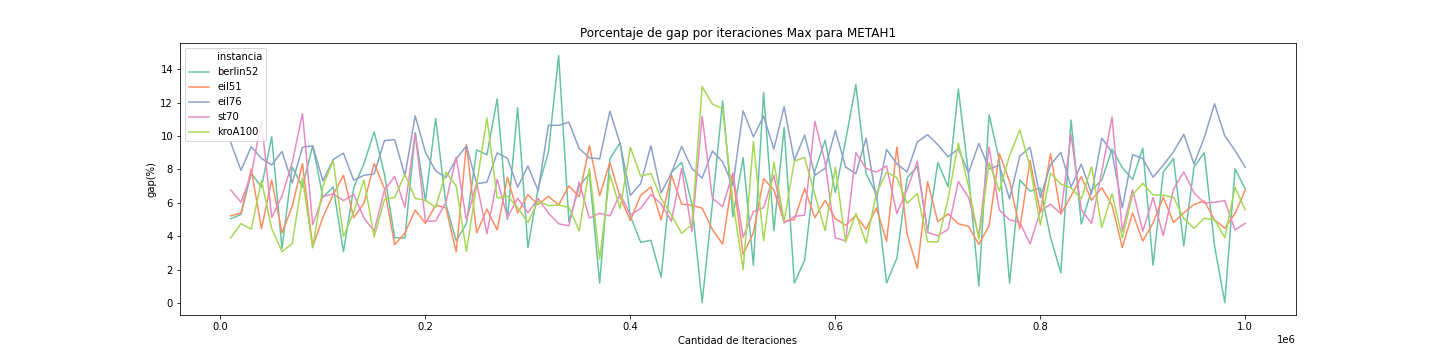
\includegraphics[scale=0.3]{Graphs-metaH/max-iter-gap-METAH1}
    \caption{Gap variando iteraciones máximas usando memoria de soluciones.}
    \label{fig:exp_maxiter_gap_metah1}
\end{figure}

\begin{figure}[h!]
    \centering
    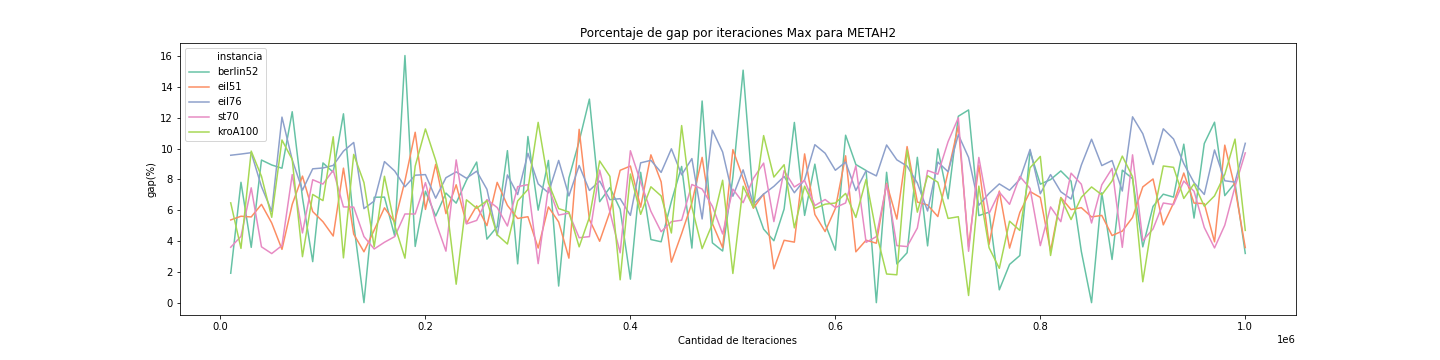
\includegraphics[scale=0.3]{Graphs-metaH/max-iter-gap-METAH2}
    \caption{Gap variando iteraciones máximas usando memoria de aristas.}
    \label{fig:exp_maxiter_gap_metah2}
\end{figure}

\begin{figure}[h!]
    \centering
    \captionsetup{justification=centering}
    \begin{subfigure}{0.45\linewidth}
        \centering
        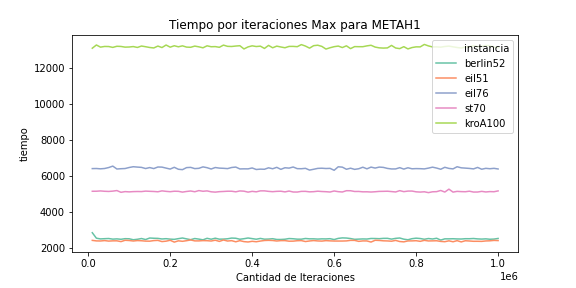
\includegraphics[scale=0.35]{Graphs-metaH/max-iter-tiempo-METAH1}
        \caption{Tiempos de ejecución variando iteraciones máximas usando memoria de soluciones}
        \label{fig:exp_maxiter_tiempo_metah1}
    \end{subfigure}
    \begin{subfigure}{0.45\linewidth}
        \centering
        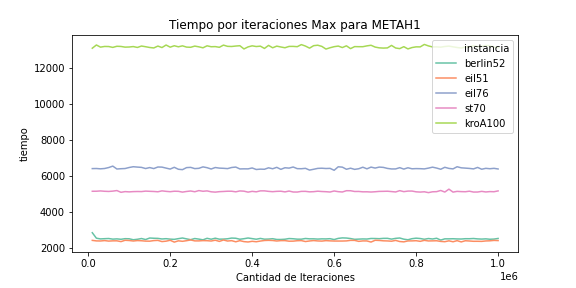
\includegraphics[scale=0.35]{Graphs-metaH/max-iter-tiempo-METAH1}
        \caption{Tiempos de ejecución variando iteraciones máximas usando memoria de aristas}
        \label{fig:exp_maxiter_tiempo_metah2}
    \end{subfigure}
    \caption{Tiempos de ejecución.}
\end{figure}

Podemos ver en las figuras \ref{fig:exp_maxiter_gap_metah1} y \ref{fig:exp_maxiter_gap_metah2} que no pareciera haber un rango de iteraciones que mejore sustancialmente la calidad de soluciones en general para las 5 instancias evaluadas. Si bien podemos encontrar mínimos locales que presentan mejoras para una instancia, no hay un valle en el gráfico que aplique para un caso general.

En las figuras \ref{fig:exp_maxiter_tiempo_metah1} y \ref{fig:exp_maxiter_tiempo_metah2} podemos ver que la cantidad de iteraciones máximas consideradas no incide sobre el tiempo de ejecución insumido por el algoritmo, esto puede deberse a que existe otro de los parámetros, un criterio de salida, que entra en acción antes que se llegue a considerar las iteraciones totales.

Como no podemos determinar un rango de iteraciones que sea claramente beneficioso para la calidad de las soluciones, vamos a quedarnos con el valor por defecto para la optimización de parámetros.

\subsubsection{Máximas iteraciones sin mejoras}
Evaluamos un rango de iteraciones desde 1000 a 100000, manteniendo los otros parámetros en los valores predeterminados mencionados anteriormente.

\begin{figure}[h!]
    \centering
    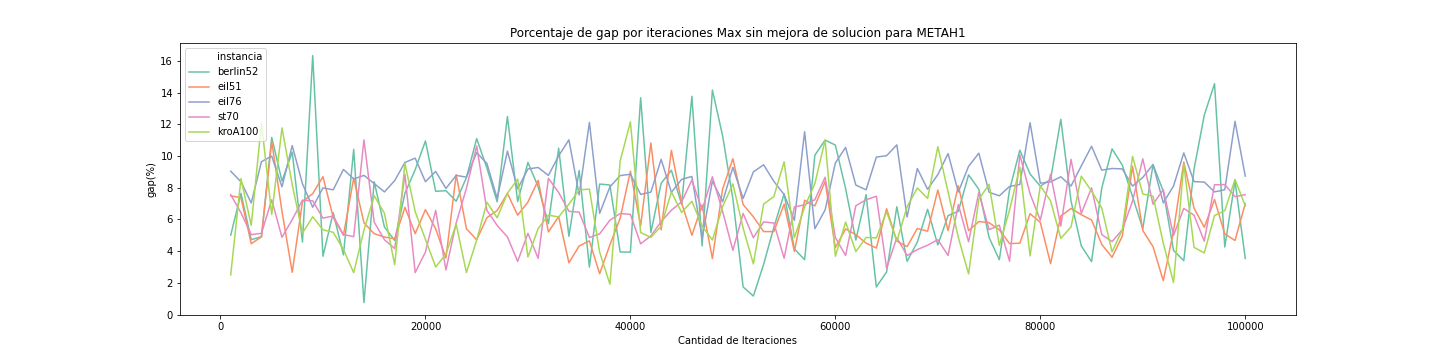
\includegraphics[scale=0.3]{Graphs-metaH/max-iter-sm-gap-METAH1}
    \caption{Gap variando iteraciones máximas sin mejora usando memoria de soluciones.}
    \label{fig:exp_maxiter_sm_gap_metah1}
\end{figure}

\begin{figure}[h!]
    \centering
    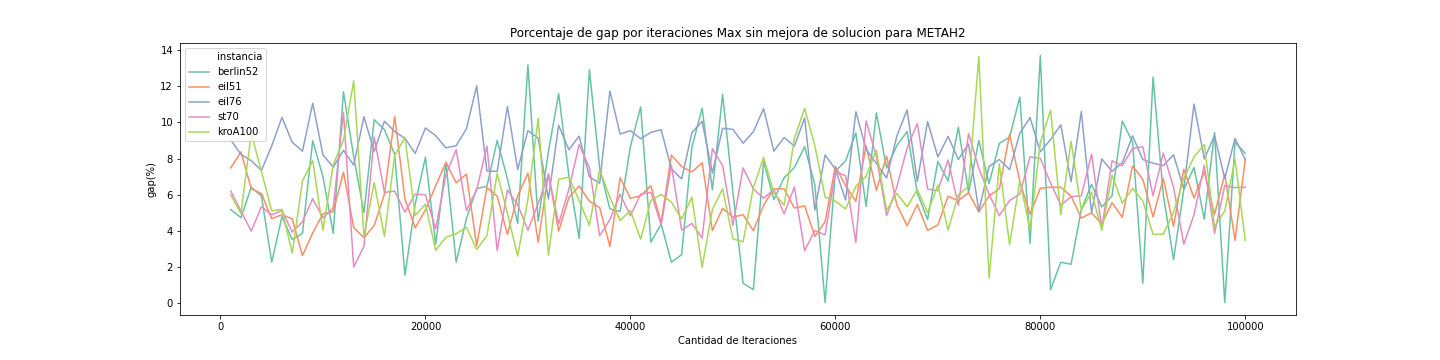
\includegraphics[scale=0.3]{Graphs-metaH/max-iter-sm-gap-METAH2}
    \caption{Gap variando iteraciones máximas sin mejora usando memoria de aristas.}
    \label{fig:exp_maxiter_sm_gap_metah2}
\end{figure}

\begin{figure}[h!]
    \centering
    \captionsetup{justification=centering}
    \begin{subfigure}{0.45\linewidth}
        \centering
        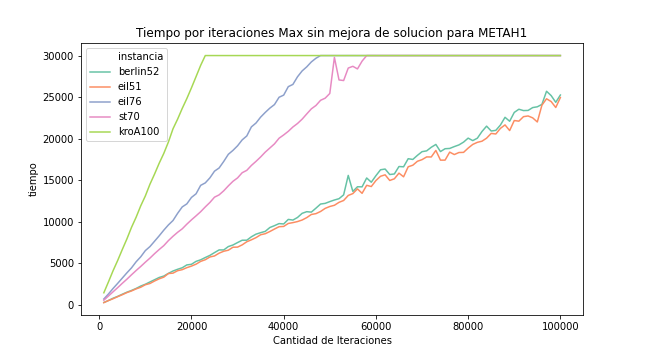
\includegraphics[scale=0.35]{Graphs-metaH/max-iter-sm-tiempo-METAH1}
        \caption{Tiempos de ejecución variando iteraciones máximas sin mejora usando memoria de soluciones}
        \label{fig:exp_maxiter_sm_tiempo_metah1}
    \end{subfigure}
    \begin{subfigure}{0.45\linewidth}
        \centering
        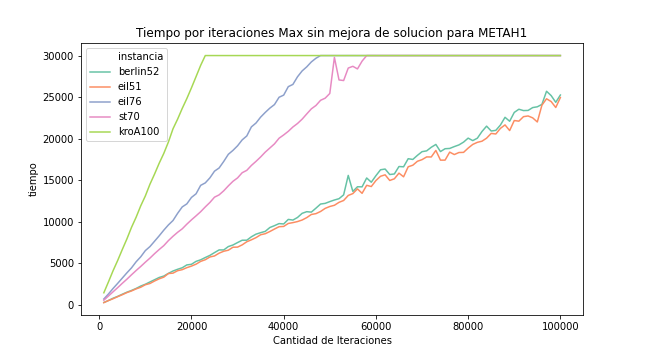
\includegraphics[scale=0.35]{Graphs-metaH/max-iter-sm-tiempo-METAH1}
        \caption{Tiempos de ejecución variando iteraciones máximas sin mejora usando memoria de aristas}
        \label{fig:exp_maxiter_sm_tiempo_metah2}
    \end{subfigure}
    \caption{Tiempos de ejecución.}
\end{figure}

Podemos ver en las figuras \ref{fig:exp_maxiter_sm_gap_metah1} y \ref{fig:exp_maxiter_sm_gap_metah2} que la calidad de las soluciones pareciera mantenerse oscilante a medida que aumenta el parámetro. Podemos ver varios rangos donde se generan valles en el gráfico que podemos considerar para elegir un buen valor de parámetro.

Sin embargo viendo las figuras \ref{fig:exp_maxiter_sm_tiempo_metah1} y \ref{fig:exp_maxiter_sm_tiempo_metah2} podemos apreciar que el tiempo de ejecución crece en proporción al aumento del parámetro hasta que chocan con el parámetro fijo de tiempo máximo. Por lo que en la elección del parámetro óptimo necesitamos la menor cantidad de iteraciones posibles que den soluciones de buena calidad.

\begin{figure}[h!]
    \centering
    \captionsetup{justification=centering}
    \begin{subfigure}{0.45\linewidth}
        \centering
        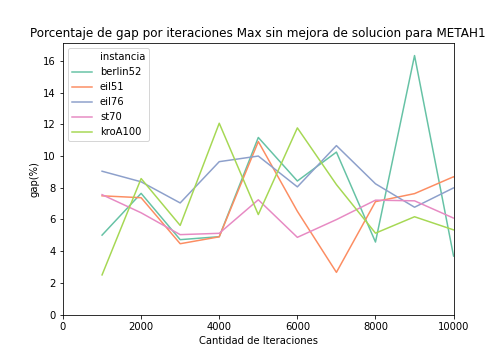
\includegraphics[scale=0.35]{Graphs-metaH/max-iter-sm-gap-METAH1-zoomed.png}
        \caption{Gap zoomeado variando iteraciones máximas sin mejora usando memoria de soluciones.}
        \label{fig:exp_maxiter_sm_gap_zoom_metah1}
    \end{subfigure}
    \begin{subfigure}{0.45\linewidth}
        \centering
        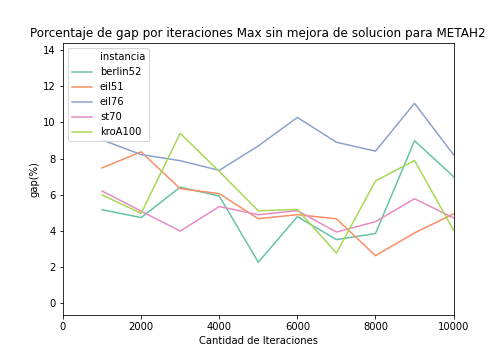
\includegraphics[scale=0.35]{Graphs-metaH/max-iter-sm-gap-METAH2-zoomed.png}
        \caption{Gap zoomeado variando iteraciones máximas sin mejora usando memoria de aristas.}
        \label{fig:exp_maxiter_sm_gap_zoom_metah2}
    \end{subfigure}
    \caption{Gap zoomeado para iteraciones sin mejora menores a 10000.}
\end{figure}

Si hacemos una ampliación de los gráficos de gap de las figuras \ref{fig:exp_maxiter_sm_gap_zoom_metah1} y \ref{fig:exp_maxiter_sm_gap_zoom_metah2} podemos ver que dentro del rango menor a 10000 iteraciones sin mejora existe un rango que tiene mínimos locales en la mayoría de las instancias experimentadas. Elegimos el valor 7500 como parámetro optimizado.

\subsubsection{Máximo tiempo de ejecución}
Evaluamos un rango de tiempo desde 1000 a 30000 milisegundos, manteniendo los otros parámetros en los valores predeterminados mencionados anteriormente.

\begin{figure}[h!]
    \centering
    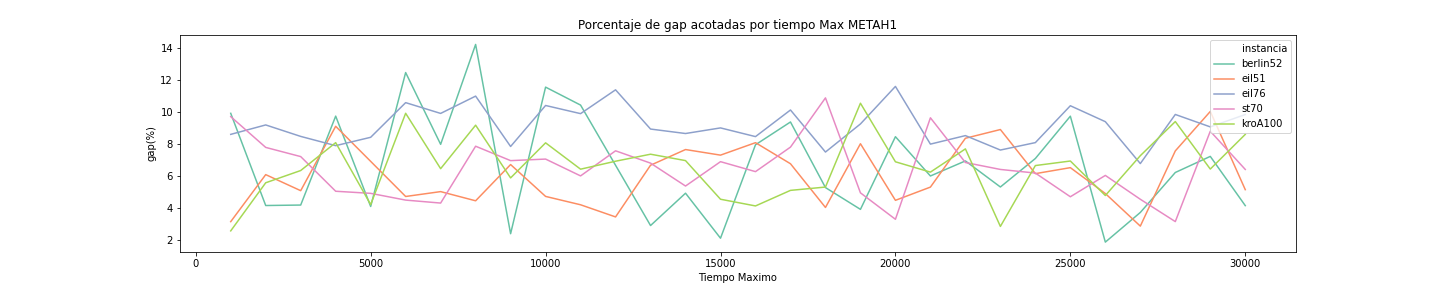
\includegraphics[scale=0.3]{Graphs-metaH/maxtime-gap-METAH1}
    \caption{Gap variando tiempo máximo usando memoria de soluciones.}
    \label{fig:exp_maxtime_gap_metah1}
\end{figure}

\begin{figure}[h!]
    \centering
    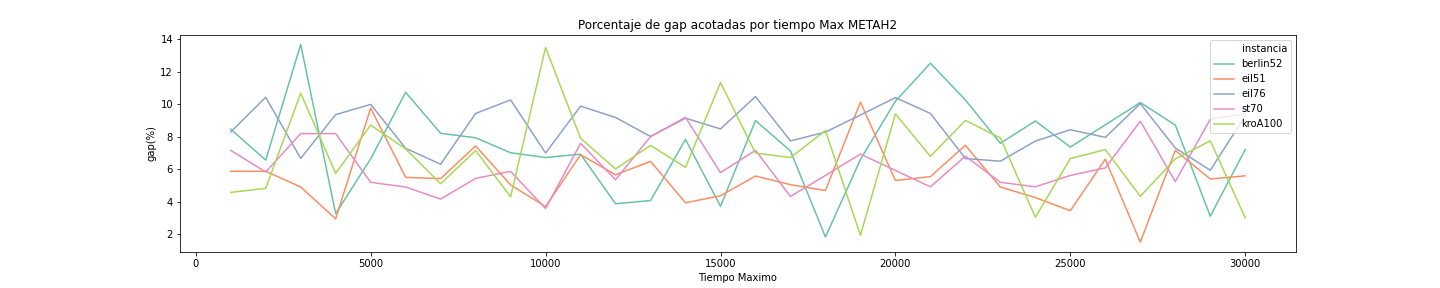
\includegraphics[scale=0.3]{Graphs-metaH/maxtime-gap-METAH2}
    \caption{Gap variando tiempo máximo usando memoria de aristas.}
    \label{fig:exp_maxtime_gap_metah2}
\end{figure}

En la Figura \ref{fig:exp_maxtime_gap_metah1} y \ref{fig:exp_maxtime_gap_metah2} vemos que los valores no nos dan mucha información acerca de una mejora del óptimo con respecto a mayor tiempo de ejecución, aunque al final de ambas gráficas se puede ver un decremento de picos altos en general, producido tal vez por el mismo aumento del tiempo para poder salir de los mínimos locales que se le administra al algoritmo.

Por otro lado a este criterio de parada no se le adjunta una gráfica del tiempo pues esta es trivial, dado que habrá una correspondencia 1 a 1 de los ejes hasta que el algoritmo se detenga por algún otro parámetro.

Sabiendo que este criterio no afecta directamente a la búsqueda del óptimo, pero si que ayuda siendo mas flexible a otros criterios de parada decidimos que un rango de tiempo máximo prudencial seria entre 15 y 20 segundos para cualquiera de los tipos de memoria.

Para la experimentación con parámetros óptimos vamos a utilizar el valor 18 segundos para el criterio de corte.

\subsubsection{Tamaño de memoria}
Evaluamos un rango de tamaño de memoria desde 1 a 50 últimas soluciones o aristas, manteniendo los otros parámetros en los valores predeterminados mencionados anteriormente.

\begin{figure}[h!]
    \centering
    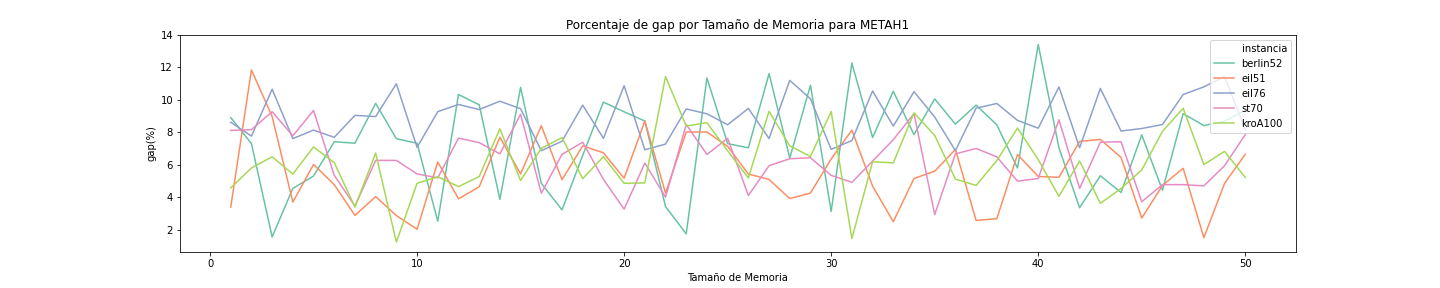
\includegraphics[scale=0.3]{Graphs-metaH/memsize-gap-METAH1.png}
    \caption{Gap variando tamaño de memoria usando memoria de soluciones.}
    \label{fig:exp_memsize_gap_metah1}
\end{figure}

\begin{figure}[h!]
    \centering
    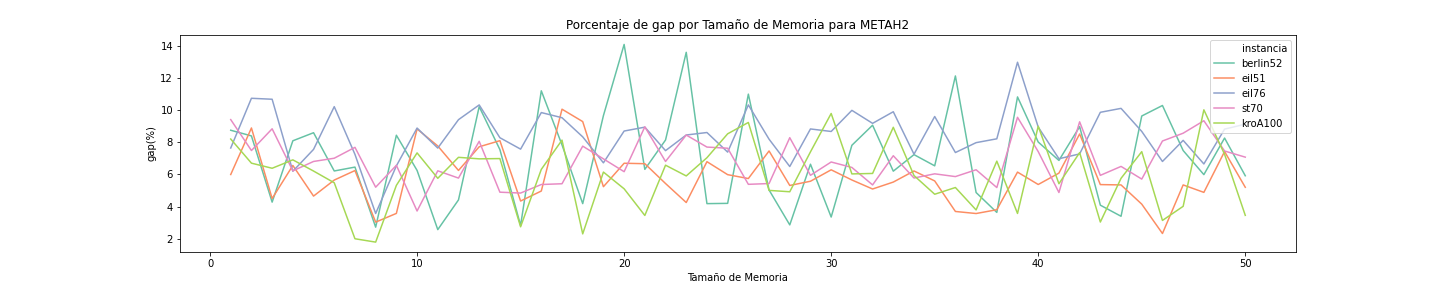
\includegraphics[scale=0.3]{Graphs-metaH/memsize-gap-METAH2.png}
    \caption{Gap variando tamaño de memoria usando memoria de aristas.}
    \label{fig:exp_memsize_gap_metah2}
\end{figure}

\begin{figure}[h!]
    \centering
    \begin{subfigure}{0.45\linewidth}
        \centering
        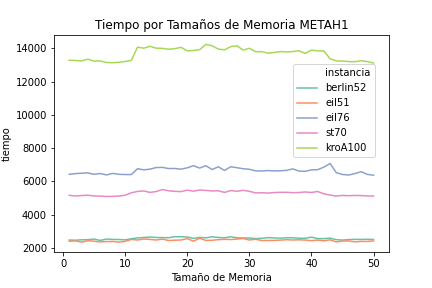
\includegraphics[scale=0.35]{Graphs-metaH/memsize-tiempo-METAH1.png}
        \caption{Tiempos de ejecución variando tamaño de memoria usando memoria de soluciones}
        \label{fig:exp_memsize_tiempo_metah1}
    \end{subfigure}
    \begin{subfigure}{0.45\linewidth}
        \centering
        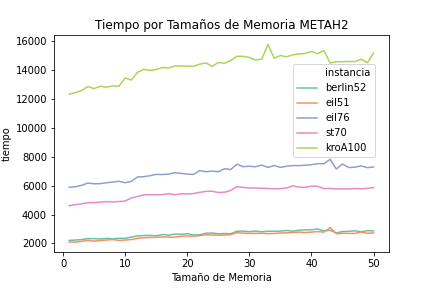
\includegraphics[scale=0.35]{Graphs-metaH/memsize-tiempo-METAH2.png}
        \caption{Tiempos de ejecución variando tamaño de memoria usando memoria de aristas}
        \label{fig:exp_memsize_tiempo_metah2}
    \end{subfigure}
    \caption{Tiempos de ejecución.}
\end{figure}

En las Figuras \ref{fig:exp_memsize_gap_metah1} y \ref{fig:exp_memsize_gap_metah2} no podemos ver demasiado información mas que un mínimo a la altura del tamaño de memoria 8 en la memoria por aristas. El resto del gráfico parece mostrar una falta de mejora con respecto al aumento del tamaño de la memoria.

Es en las Figuras \ref{fig:exp_memsize_tiempo_metah1} y \ref{fig:exp_memsize_tiempo_metah2} donde tenemos una mejora mientras mas bajo sea el tamaño de ambas memorias, para METAH2 tenemos un empeoramiento lento progresivo del tiempo insumido a mayor tamaño de memoria, con algunos saltos en el medio. En cambio para METAH1 tenemos un salto de tiempo a partir del tamaño 10 aproximadamente, el cual se estabiliza hasta el tamaño 40, y luego vuelve a bajar.

Acompañado del análisis de los gaps decidimos que un buen parámetro final para este parámetro seria el tamaño de memoria configurado en 8, dado que se encuentra antes de los saltos mencionados para el consumo de tiempo y porque luego del 10 el consumo de tiempo aumenta en ambas memorias.
%COMPLETAR si creen necesario con mas info, o cambiar la conclusion%

%---------Deje el grafo zoomeado en tamaño 0-10 comentado por si creen que podemos agregarlo
% \begin{figure}[h!]
%     \centering
%     \captionsetup{justification=centering}
%     \begin{subfigure}{0.45\linewidth}
%         \centering
%         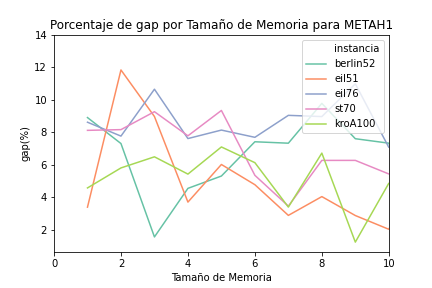
\includegraphics[scale=0.35]{Graphs-metaH/memsize-gap-METAH1-zoomed.png}
%         \caption{Gap zoomeado variando el tamaño de la memoria de soluciones.}
%         \label{fig:exp_memsize_gap_zoom_metah1}
%     \end{subfigure}
%     \begin{subfigure}{0.45\linewidth}
%         \centering
%         \includegraphics[scale=0.35]{Graphs-metaH/memsizegap-METAH2-zoomed.png}
%         \caption{Gap zoomeado variando el tamaño de la memoria de aristas.}
%         \label{fig:exp_memsize_gap_zoom_metah2}
%     \end{subfigure}
%     \caption{Gap zoomeado para iteraciones sin mejora menores a 10000.}
% \end{figure}


\subsubsection{Porcentaje de vecindad}
Evaluamos un rango de tamaño de vecindad considerada desde 10\% a 50\%, manteniendo los otros parámetros en los valores predeterminados mencionados anteriormente en la sección \ref{exp-parametros}. Como la selección de elementos que ingresan a esa vecindad es aleatoria, tener un rango que minimice el gap no garantiza que sea así en todas las ejecuciones, por este motivo buscamos un gap que sea robusto en general tratando de que los picos máximos de gap sean lo más bajo posible para todos los casos.

\begin{figure}[h!]
    \centering
    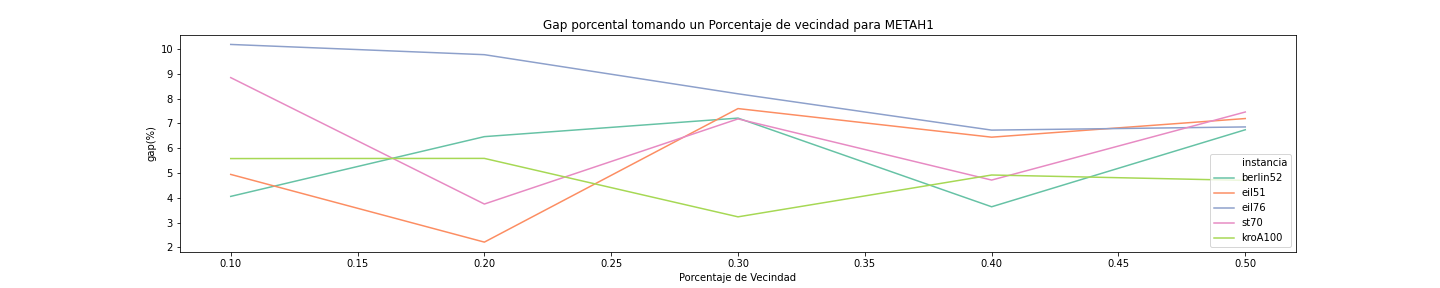
\includegraphics[scale=0.3]{Graphs-metaH/vecindad-gap-METAH1.png}
    \caption{Gap variando porcentaje de vecindad usando memoria de soluciones.}
    \label{fig:exp_porc_gap_metah1}
\end{figure}

\begin{figure}[h!]
    \centering
    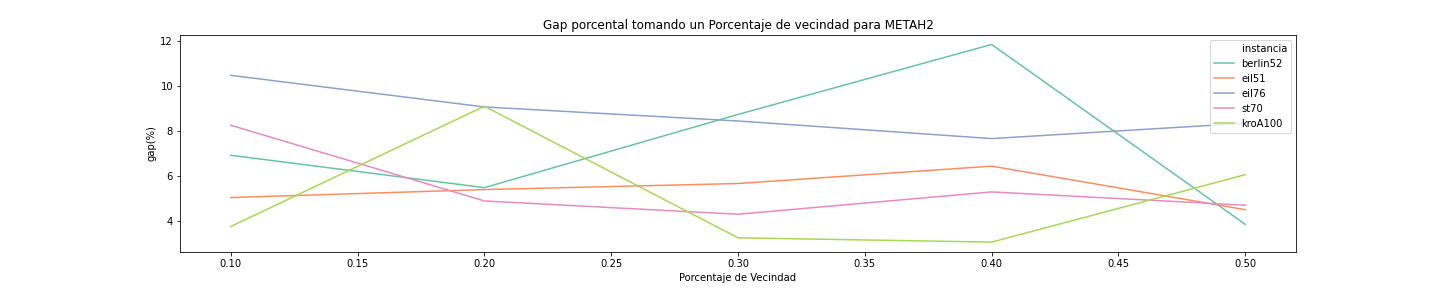
\includegraphics[scale=0.3]{Graphs-metaH/vecindad-gap-METAH2.png}
    \caption{Gap variando porcentaje de vecindad usando memoria de aristas.}
    \label{fig:exp_porc_gap_metah2}
\end{figure}

\begin{figure}[h!]
    \centering
    \begin{subfigure}{0.45\linewidth}
        \centering
        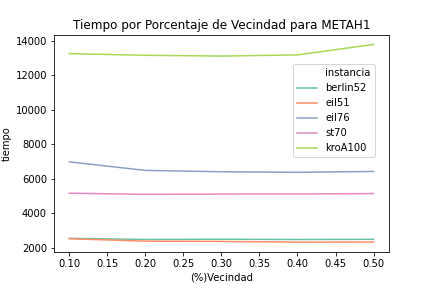
\includegraphics[scale=0.35]{Graphs-metaH/vecindad-tiempo-METAH1.png}
        \caption{Tiempos de ejecución variando porcentaje de vecindad usando memoria de soluciones}
        \label{fig:exp_porc_tiempo_metah1}
    \end{subfigure}
    \begin{subfigure}{0.45\linewidth}
        \centering
        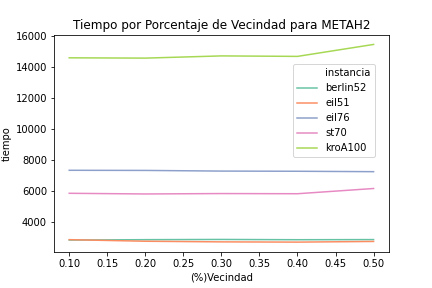
\includegraphics[scale=0.35]{Graphs-metaH/vecindad-tiempo-METAH2.png}
        \caption{Tiempos de ejecución variando porcentaje de vecindad usando memoria de aristas}
        \label{fig:exp_porc_tiempo_metah2}
    \end{subfigure}
    \caption{Tiempos de ejecución.}
\end{figure}

Notamos que en las figuras \ref{fig:exp_porc_tiempo_metah1} y \ref{fig:exp_porc_tiempo_metah2} el valor del parámetro porcentaje de vecindad no condiciona sustancialmente el tiempo de ejecución del algoritmo.

Podemos ver en las figuras \ref{fig:exp_porc_gap_metah1} y \ref{fig:exp_porc_gap_metah2} que no parece haber un valor que favorezca a las todas las instancias en general, valores como \%20 parecen ser mejores para 'eil51' y 'st70' pero son malos para 'eil76' y 'kroA100'. Esta última 'kroA100' tiene su óptimo en los \%30 pero es el peor valor para las demás. Si consideramos como cota superior el valor máximo entre las instancias para un mismo porcentaje podemos observar que \%50 no tiene el mejor gap para las instancias en particular pero tiene un gap menor a \%8 para todas las instancias, lo que lo hace un parámetro robusto para la mayoría de los casos evaluados, siempre que sea aceptable el gap de \%8 para la solución. Para la optimización de parámetros seleccionamos este valor de \%50.

\subsection{Evaluación de parámetros encontrados}
Finalmente vamos a evaluar los parámetros obtenidos durante la experimentación anterior sobre un nuevo set de instancias 'rat195', 'rat575' y 'rat783' ya mencionada en la sección \ref{sec:exp-instancias}, con la idea de verificar que efectivamente llegamos a buenos parámetros que nos permiten llegar a una solución de calidad sobre una instancia diferente a las consideradas para evaluar cada parámetro individualmente.
Los parámetros óptimos obtenidos en la sección anterior fueron los siguientes:
\begin{itemize}
    \setlength\itemsep{-0.4em}
    \item maxiter: 100000.
    \item maxiter-sm: 7500.
    \item maxtime: 18 seg.
    \item memsize: 8.
    \item porc: 0,5 (50\%).
\end{itemize}

Ejecutamos nuevamente las metaheurísticas sobre la instancia 'rat195' y obtenemos que ambas implementaciones (memoria de soluciones o de aristas) cortan a los 18 segundos parametrizados como criterio de parada.
\begin{itemize}
    \item Gap usando memoria de ciclos: \%6,99
    \item Gap usando memoria de aristas: \%6,22
\end{itemize}

Podemos observar que los parámetros prefijados durante la experimentación anterior dieron una solución aceptable considerando un gap menor a 7\% respecto al óptimo real.
Sabiendo que el proceso fue frenado por el criterio de parada de 18 segundos hipotetizamos que de haber seleccionado un tiempo parámetro más alto es probable que encontremos mejores soluciones.

Ejecutamos nuevamente el experimento sobre 'rat195' pero cambiando el parámetro de tiempo de parada por 30 segundos.
\begin{itemize}
    \item Gap usando memoria de ciclos: \%6,70
    \item Gap usando memoria de aristas: \%6,04
\end{itemize}

En este caso la diferencia de tiempo de parada no influyó fuertemente en la calidad de la solución, siendo que aumentamos el parámetro de 18 a 30 segundos pero solamente conseguimos mejoras de gap de \%0.20 aproximadamente. Por lo que el parámetro de tiempo seleccionado parece dar una buena relación tiempo/calidad. Estos resultados pueden ser vistos en la Figura \ref{fig:exp_dif_gap_rat195}.

\begin{figure}[h!]
    \centering
    \begin{subfigure}{0.45\linewidth}
        \centering
        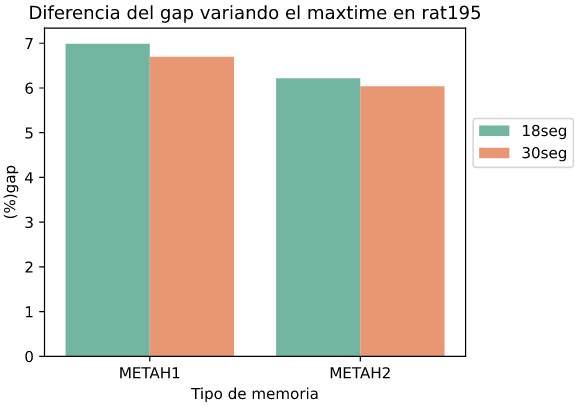
\includegraphics[scale=0.30]{Graphs-punto5/punto5-rat195.png}
        \caption{Diferencia de porcentaje de gap en la instancia 'rat195' usando distintos tiempos maximos}
        \label{fig:exp_dif_gap_rat195}
    \end{subfigure}
    \begin{subfigure}{0.45\linewidth}
        \centering
        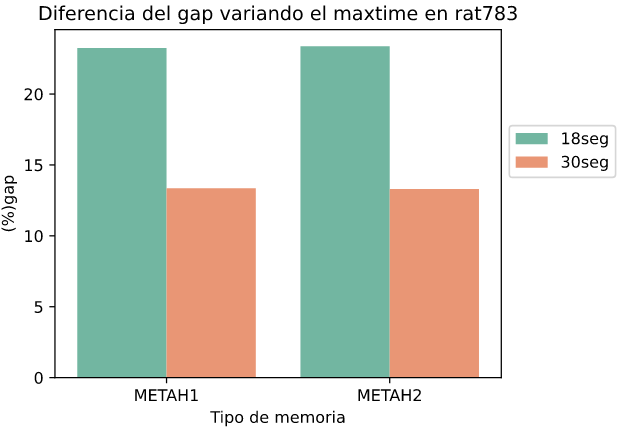
\includegraphics[scale=0.29]{Graphs-punto5/punto5-rat783.png}
        \caption{Diferencia de porcentaje de gap en la instancia 'rat783' usando distintos tiempos maximos}
        \label{fig:exp_dif_gap_rat783}
    \end{subfigure}
    \caption{Tiempos de ejecución.}
\end{figure}

Luego probamos el algoritmo sobre instancias de tamaño mayor que las evaluadas durante la experimentación de parámetros con el objetivo de probar la hipótesis de que los parámetros seleccionados son "buenos" para instancias de tamaños similares a las evaluadas.

Evaluamos sobre la instancia 'rat575' donde vimos resultados muy similares a los de la instancia anterior, con un gap de aproximadamente \%9,19 y \%9,85 para la memoria de ciclos y la de aristas respectivamente, con mejoras de aproximadamente un \%1.5 al aumentar el tiempo máximo a 30 segundos para ambos tipos de memoria.

Por ultimo ejecutamos nuevamente el experimento sobre 'rat783' manteniendo los parámetros obtenidos anteriormente. En este caso también corta el algoritmo por los 18 segundos parametrizados de criterio de parada.
\begin{itemize}
    \item Gap usando memoria de ciclos: \%23,24
    \item Gap usando memoria de aristas: \%23,37
\end{itemize}
Luego probamos aumentando el tiempo máximo a 30 segundos para ver si había una mejora que sea considerable.
\begin{itemize}
    \item Gap usando memoria de ciclos: \%13,36
    \item Gap usando memoria de aristas: \%13,30
\end{itemize}
Como nos muestra la Figura \ref{fig:exp_dif_gap_rat783} con los parámetros optimizados en esta instancia mucho mas grande, obtuvimos que con un tiempo máximo mas chico limitamos la posibilidad de que se encuentre una mejor solución. Esto es justificable dado que las instancias con las que trabajamos originalmente eran mucho menores que la que estamos analizando en este momento.

Corroboramos que la calidad de los parámetros seleccionados depende del tamaño de la instancia sobre la que se ejecuta el algoritmo. En el caso de 'rat783' tenemos una instancia de tamaño casi 4 veces el de 'rat195' y se puede observar que con los mismos parámetros, el gap da \%18 aproximado de diferencia negativa.

Podemos concluir que los parámetros obtenidos dan buenos resultados en instancias de tamaño similares a las evaluadas, pero dejan de ser efectivos para otras instancias de tamaños diferentes o con diferentes requerimientos de precisión respecto a la solución óptima.

\newpage
\section{Conclusiones}
El TSP es un problema relevante en el mundo real, con repercusiones de millones de dólares en la industria, sin embargo, por su naturaleza NP-Hard y el costo computacional de resolverlo no existe un algoritmo por defecto, más eficiente o más rápido de uso genérico, sino al contrario la elección del mismo depende de las necesidades del problema y las compensaciones (o \emph{tradeoff}) que se estén dispuestas a asumir. Desde el marco de esta investigación se tomo la solución exacta como muy costosa en términos de tiempo (aún utilizando técnicas de programación lineal entera), y se optó por estudiar una familia de heurísticas con una cota temporal mas eficiente y de complejidad polinomial determinista. Se evaluó cada una y se compararon entre si, mientras a su vez se experimentó con meta-heurísticas para mejorar la calidad de la solución y disminuir el gap entre el resultados obtenido con respecto al óptimo del problema. Además, se realizaron experimentos sobre los parámetros de las meta-heurísticas en cuestión para conseguir la mayor eficiencia posible en las instancias de interés evaluadas. %: grafos que representen la cantidad de entregas en un día por camión de envíos (aproximadamente 130 vértices según estadistas de UPS). 

En la experimentación de las heurísticas más simples, la de vecino más cercano (HVMC) obtuvo una buena relación tiempo, calidad de la solución, además de ser un algoritmo de fácil desarrollo y baja complejidad. Sin embargo aunque existen familias particulares de instancias en las cuales se pueden acotar el gap de la solución, en el caso genérico no existen garantías para este algoritmo por lo cual se recomiendan otras heurísticas en casos donde importe más garantizar una mejor solución que el tiempo de cómputo. 
En el caso de la arista más cercana (HAMC) ocurre lo contrario, presentando una buena solución en la mayoría de los experimentos pero con un costo de tiempo mucho mayor, por lo cual en casos donde el tiempo es muy limitado y la calidad de la solución no es tan relevante se recomienda la primera heurística. Por último, está la HAGM que aunque no tuvo el desempeño mas rápido, ni la mejor solución tuvo un rendimiento intermedio, y en especial permite definir una cota del gap para el caso genérico (vale porque los grafos de distancias son euclidianos) al ser 1-aproximado y es por esta garantía es que se le eligió esta heurística para aplicar las meta-heurísticas sobre su solución. En futuras investigaciones más avanzadas se recomienda replicar los experimentos utilizando heurísticas con cotas del gap mas chicas (aunque mas complejas de implementar) como el algoritmo de Christofides y Serdyukov que es 1/2-aproximado.

Se iteró de forma experimental sobre los diferentes parámetros de las meta-heurísticas con memoria tanto por soluciones como por aristas y se encontraron valores que buscan minimizar el gap de la solución de manera aceptable y suficiente para la expectativa del estudio en las instancias esperadas (no masivas, entre 50 y 100 vértices). 
%Aunque existen casos adversos como en todo algoritmo estos son muy difíciles de encontrar en el mundo real, y el carácter aleatorio del algoritmo al buscar por vecindad disminuye aun más la posibilidad de generar resultados muy distantes del óptimo, y 
Para las pruebas finales una vez elegidos los parámetros, se obtuvo buenos resultados para otras instancias de prueba de similar tamaño, sin embargo como se esperaba para las instancias grandes con más de 500 vértices, el gap fue mayor (posiblemente porque los parámetros fueron evaluados y seleccionados en instancias de tamaños mucho menores), sin embargo el estudio de esta cantidad de vértices escapa de las posibilidades de realizar experimentaciones en tiempos considerables para este trabajo práctico. 

La selección de los parámetros que optimizan la meta-heurística está condicionada por las características de las instancias evaluadas por lo que es difícil o quizás imposible fijarlos de forma general. De ser usado el algoritmo se deberá primero analizar la instancia, y tratar de deducir los parámetros individuales que benefician esa ejecución en particular. El presente trabajo deja propuesto parámetros para las instancias estudiadas de entre 50 y 200 vértices.

Finalmente aunque ambas meta-heurísticas proporcionan buenos resultados, en casos donde la cantidad de memoria disponible es una limitante se recomienda el uso de meta-heurística de memoria por aristas ya que su consumo en espacio es menor que el utilizando en memoria por soluciones completas. 

\newpage
\bibliographystyle{unsrt}
\bibliography{bibliografia}

\end{document}